% Summary of the workshop session: 
% Science Goals Requiring Community Brokers and related unconference sessions. 

\section{Science Drivers (Melissa)} \label{sec:science}

\LPG[inline]{It would be good to see a table of the timescale demanded for access to alerts by all science cases, similar to what Ashley presented for TVSSC, but for all science goals }

\noindent
{\it Section Status: draft in progress. \\
To Do: \\
Section could be shortened by gathering all the "broker needs" and "problems forseen" from each subsection into a single collated subsection (\S~\ref{ssec:sci_sum}). MLG can do this later. \\ 
Invite the original presenters to review text and be coauthors.\\
Include any other science drivers from the other talks and unconferences.\\ Ensure this section is adequately answering the questions: \\
 - Which science drivers need community brokers and follow-up? \\
 - Which science drivers need the LSST prompt data products (60s and 24h latency)?  \\
 - Which science cases require new approaches? \\
 - What do the LSST science collaborations want to see from community brokers? \\

\LPG[inline] {Suggest to add in a discussion of some of the scientific challenges for LSST alerts; Contrast the luxury of Catalina, which is able to optimize to one science goal to the challenges of LSST, which must accommodate a multitude of science goals}
}

\medskip
This section summarizes the invited presentations from each of the LSST Science Collaborations (SC), which addressed the science drivers that rely on working with the LSST alert stream and/or prompt data products. One of the goals of this session was to ensure that broker developers are informed of the variety of science goals for LSST Prompt products, so that they can develop systems that respond to the science needs. A full overview of LSST science drivers are detailed in the LSST overview paper \cite{2019ApJ...873..111I} ({\bf cite also the science book}).



\subsection{Transients and Variable Stars}\label{ssec:sci_tvs}
% Rep: Ashley Villar
% Material sourced from:
% LSST CBW Participants Drive > Presentations - Wednesday Afternoon > Slides for SC Rep Talks at LSST CBW (TVS)
% LSSTBrokerWorkshop19 > SOC's Notes (private)

The Transients and Variable Stars (TVS) Science Collaboration is focused on studies of intrinsically variable events (periodic and aperiodic), explosive and eruptive transients, as well as extrinsic variables and transients (e.g., eclipsing binaries, microlensing). Science goals include both improving the physical understanding of these systems (e.g., stellar evolution, high-energy astrophysics) and using these objects as distance markers and probes of their environment (e.g., mapping the Milky Way, characterizing the intracluster medium, and dark energy cosmology). The objects which fall under the TVS umbrella span a wide range of timescales and energy outputs, and their studies frequently involve multi-messenger (e.g., neutrinos, gravitational waves) and/or multi-wavelength observations that span the electromagnetic spectrum. 

Some of these TVS science goals require the alerts (and brokers) in order to categorize objects and identify those which need rapid follow-up (e.g., spectroscopy, multi-band photometry) to provide the definitive classification and/or key astrophysical evidence. For example, finding young supernovae within hours of explosion when the optical and near-ultraviolet spectrum exhibit the short-lasting signatures of shock breakout (which can constrain the radius of the progenitor star; {\bf reference}), identifying a $\lesssim$day-long exoplanet feature in a microlensing event, or discovering optical counterparts to gravitational wave events. 

Other TVS science goals which need follow-up on longer time scales (days to weeks) could technically use the Prompt products database (PPDB; {\bf reference paper section}) instead of alerts, but may use the alerts and brokers system infrastructure for classification anyway. For example, identifying supernovae that are nearing peak brightness in order to make the most efficient use of spectroscopic classification resources, or determining when an eclipsing binary has passed a quality threshold (e.g., orbital parameter errors have decreased below a limit) to warrant follow-up. In a survey of the TVS members' needs for alerts and brokers ({\bf how to reference Rachel's report?}), responses to a question about access to difference-image sources were about evenly divided between ``same-night" and ``three days or longer". Respondents were also about equally divided between wanting alerts delivered by VOEvent stream and API subscriber, (more immediate use) or by an online page or email, corresponding to desires for more immediate use and a longer latency, respectively.

Given the diversity of TVS use-cases for an LSST alert broker, there is also a diversity of needed features. Simple filtering -- applying limits on the alert packet contents -- is insufficient for many of the TVS science goals mentioned above, which require several value-added processes. In particular, associating same-night alerts for a new source is necessary to provide a color\footnote{Recall that alerts are issued for sources detected in a single difference-image, and if a source is new and not yet in the PPDB, none of its alerts during its first night of detection will contain association information.}, light-curve fits to and/or feature extraction from the historical data in the alert packet are necessary for categorization, and cross-matching with external catalogs and/or a robust evaluation of host galaxy offset\footnote{The identification of a host galaxy is not always simply the nearest static-sky source, but requires a probabilistic assessment of the offset in effective radii and other galaxy attributes.} are needed for additional contextual information in prioritizing follow-up. The TVS has also identified the science-driven need to characterize the selection biases of brokering systems, which may entail giving users the ability to generate and process simulated events, and the need to broker (or re-broker) alerts from past events (e.g., when an algorithm is updated). 

Triggering follow-up is at the core of TVS's alert-based science goals, and for that, broker systems which facilitate the activation of Target of Opportunity observations are needed -- whether it be by notifying a human, automatically submitting packets to queue-scheduled facilities, or directly scheduling observations with robotic telescopes. Some or all of this triggering process might not happen within the broker, but instead within Target Observation Managers ({\bf reference section of this paper}) to which brokers connect -- and thus interfacing with TOMs is another science-driven need from the TVS perspective.

{\bf Challenges Faced --} First, it is acknowledged that some of the science-driven broker needs, such as feature extraction and processing simulated streams, will require considerable computational resources. Second, obtaining robust categorizations for objects with sparsely sampled light-curves, especially during the hours and days following the start of a photometric event, remains an open challenge. So does identifying the rare and unexpected ``needles in a haystack" -- without yet knowing exactly the characteristics of the needles! -- that LSST will be uniquely able to discover. In both cases the community is actively working on algorithm development ({\bf \ref{sec:algorithms}}). Third, creating TOMs which enable both rapid follow-up, and the construction of highly curated target lists to optimize the use of scarce follow-up resources, is a non-trivial aspect that the community is also actively working towards ({\bf cite TOMs section}).

\subsection{Solar System}\label{ssec:sci_ss}
% Rep: Lynne Jones
% Material sourced from:
% LSST CBW Participants Drive > Presentations - Wednesday Afternoon > Jones_SSSC_rep.pdf
% LSSTBrokerWorkshop19 > SOC's Notes (private)

The Solar System Science Collaboration (SSSC) focuses on studies of small bodies, asteroids and minor planets, such as finding and cataloging the near-earth asteroid (NEO) population for impact risk assessment, studying outbursts and emissions from asteroids, and building and characterizing the populations of the outer solar system like Kuiper Belt Objects (KBOs). In images, the SSSC's objects of interest can appear as point, trailed, or extended sources. Multiple images separated by at least 30 minutes (and up to days) are required to confirm newly discovered moving objects that appear as point sources in individual images\footnote{For the faintest KBOs, sources are not detected in individual images and require shift-and-stack processing, but that is not a part of Prompt processing and does not lead to alerts.}. Longer-term photometric monitoring is required to characterize rotation, identify binary companions, and provide context for outbursts and activity. 

The SSSC plans to use LSST alerts for those studies in two main ways. One way is to discover very fast moving objects such as NEOs, potentially hazardous asteroids (PHAs), and interstellar objects (e.g., 'Oumuamua; \citealt{Meech2017}). This would be done by linking alerts from multiple images in a given night, or from a single image if the object moves during an exposure and appears trailed, in order to trigger immediate follow-up observations to constrain the orbital parameters and photometric variability. The second way is to identify outbursts from sudden changes in size or brightness, and trigger immediate follow-up. 

These SSSC use cases for alerts would be enabled by brokers that can: (1) filter on the size and shape parameters measured for all difference image sources and included in the alerts; (2) associate the detections of previously unknown moving objects that appear in multiple images during the night; (3) support access to the postage stamp LSST images; (4) maintain databases of solar system objects in order to associate new LSST alerts and update orbits in real time (especially for fast-moving objects); and/or (5) offer API ``pull" and ``push" functionality for, e.g., hourly orbit database updates or high-priority follow-up needs, respectively. Furthermore, direct connections with TOMs with web-based user interfaces to build samples, perform analysis, and vet targets for follow-up was also noted as highly desirable for solar system studies. 

{\bf Challenges Faced --} There are several items identified by the SSSC that are in need of work in order to achieve their alerts-related science goals in the LSST era, such as: 
the reliable identification of outburst activity; 
fitting light curves with sparse data points (in common with TVS); 
error calculations for orbital predictions and ephemerides; 
visualization tools for large populations of objects; 
searches of pre-existing survey data for newly discovered solar system objects; and
optimizing follow-up resources ({\bf cite NEOfixer and the Catalina talk}).


\subsection{Stars, Milky Way, and Local Volume}\label{ssec:sci_smwlv}
% Rep: Jennifer Sobeck
% Material sourced from:
% LSST CBW Participants Drive > Presentations - Wednesday Afternoon > JS_SC_SMWLV_Presentation.pdf
% LSSTBrokerWorkshop19 > SOC's Notes (private)

The main LSST science goals of the Stars, Milky Way, and Local Volume (SMWLV) Science Collaboration are to understand the structure and assembly history of the Milky Way and Local Volume galaxies --- including the role of streams, clusters, bulges, arms, and dwarf satellites --- and the fundamental physical properties of stars within several hundred parsecs of the Sun. This will be done by building multi-dimensional maps from the LSST astrometric and photometric data which include position, kinematics, brightness, color, metallicity, and variability information. 

Although much of the SMWLV science goals will use the static-sky Data Release data products ({\bf cite, e.g., dpdd?}), in cases where follow-up with external resources is required to enable variability-related studies, the Prompt products -- and sometimes the alerts in particular -- will also be used. For example, studies of cataclysmic variables, eclipsing binaries, microlensing events, and stellar flares, outbursts, or magnetic activity.
%%% of high proper-motion stars which are faint but nearby, or perhaps were kicked from stellar systems
For a broker to enable SMWLV science goals they should thus consider providing: 
(1) photometric classification of variable stars;
(2) light curve feature extraction and period determination;
(3) cross-matching to external catalogs (e.g., to identify X-ray binaries); and
(4) the ability to coordinate follow-up observations (or link with a TOM). 

{\bf Challenges Faced --} The main issues regarding alerts-related science that are currently being faced by the SMWLV team are: 
developing algorithmic components for light curve classification;
identifying anomalous star behavior in need of follow-up; 
deblending techniques stars in crowded fields; and
source association and cross-matching with external catalogs.
In addition, TOM systems that can handle large populations, reprioritize targets in real time, and automatically provide coordinates to, e.g., fill spare fibers of a MOS on an as-needed basis, would facilitate alerts-related SMWLV science. It was also noted that all of this takes time and funding, the lack of which is a significant barrier to progress.

\subsection{Dark Energy}\label{ssec:sci_desc}
% Rep: Rahul Biswas
% Material sourced from:
% LSST CBW Participants Drive > Presentations - Wednesday Afternoon > DESC_rbiswas
% LSSTBrokerWorkshop19 > SOC's Notes (private)

The primary goal of the Dark Energy Science Collaboration (DESC) is to perform a standalone stage IV dark energy experiment with the LSST data, using a full suite of cosmological probes such as weak lensing, galaxy clustering, supernovae (SNe), strong lensing, and baryon acoustic oscillations. The time-domain aspects of DESC's science goals are SNe and strong lensing, and are thus the most likely to use alerts. 

To build a Hubble diagram the DESC aims to assemble a large sample of light curves for Type Ia supernovae (SNe\,Ia), which are standard{\it izable} candles that serve as cosmological distance indicators. This science requires well-sampled multi-band light curves for all objects, and spectroscopic confirmation of their type for at least a subset. Since SNe\,Ia have a $\gtrsim$2 week-long rise time, triggering this kind of follow-up can have a latency of days to weeks. It may be that alerts are not generally necessary, and that the Prompt source catalogs are sufficient for DESC's SN\,Ia science goals --- with some possible exceptions. For example, at early-times the SN\,Ia emission exhibits behavior that may be particularly constraining of the progenitor star and/or explosion mechanism\footnote{E.g., the distribution of $^56$Ni, or the presence of circumstellar material or a giant binary companion; {\bf MLG get citations}.} -- information that may improve the standardization of SN\,Ia light curves, but requires rapid triggers for multi-band photometry and/or spectroscopic follow-up. In this case, a broker would expedite this follow-up. The DESC science goal of SN\,Ia cosmology also requires a robust understanding of the selection biases in the sample.

Most of the other SN-related science goals of DESC, e.g., as indicators of galaxy peculiar velocities, weak lensing magnification, and strong gravitational lensing, all have needs and timescales that are similar to SN\,Ia cosmology with respect to follow-up and broker usage. One exception is the search for electromagnetic counterparts of gravitational wave events, which provide cosmological information. This is one science goal where the time scale is short (hours) and alerts are the optimal -- but it does not require the robust understanding of selection biases in the filters and algorithms. In addition, searches for strongly lensed sources is facilitated with access to the images, either via the postage stamps in the alerts or via access to the Prompt products' images. For all time-domain science, in order to make optimal use of scarce follow-up resources such as spectroscopy, it is desirable to prioritize SN candidates based in part on the likelihood of LSST obtaining future observations and generating a usable light curve. 

If DESC does decide to use alerts for its time-domain cosmology studies, the broker features which would best facilitate the science are: 
(1) cross-matching to external catalogs (e.g., for host galaxy identification);
(2) well-characterized filters and algorithms;
(3) provenance for all output data;
(4) support for version control with the ability to simulate reprocessing the stream at any point in the past; 
(5) support for postage stamp analysis; and
(6) the ability to incorporate LSST forecast observations into candidate evaluations.

{\bf Challenges Faced --} As described in ({\bf cite DESC LONI section here}), DESC is actively working to assess which science goals are best met with the Prompt products and which will require alerts and brokers. Working with members of the other science collaborations to share code and derived data products, to reduce redundancy in effort and enable more science, is also an area of interest. 

\subsection{Active Galactic Nuclei}\label{ssec:sci_agn}
% Rep: Paolo Coppi
% Material sourced from:
% LSST CBW Participants Drive > Presentations - Wednesday Afternoon > coppi_agnsc_lsstbroker4.pdf
% LSSTBrokerWorkshop19 > SOC's Notes (private)

The main science goal of the Active Galactic Nuclei (AGN) Science Collaboration is to select 20-50 million AGN from among the billions of LSST galaxies, and characterize their brightness, color, and variability (on timescales from minutes to decades), in order to understand AGN evolution as a function of cosmic time, host galaxy type, larger environment, mergers and interactions, etc. Multi-wavelength studies that include, for example, radio properties, high-energy emission, and spectral emission lines, are necessary for comprehensive studies of the physics driving the AGN emission (e.g., reverberation mapping). Like other astrophysical phenomena, AGN studies benefit from multi-wavelength observations that are co-temporal (or nearly). Since the timescale of AGN variability is driven by the size of the emitting material, and/or the orbital period in the case of binary black holes, obtaining follow-up within days to weeks is typically sufficient for most AGN science, and so alerts might not be strictly necessary. One exception might be instances of dormant black holds flaring due to the tidal disruption of stars, planets, or gas clouds -- of which LSST might find $\sim$1000 per year -- are important to catch early on, because physical information about, e.g., relativistic jets is revealed within the first day(s). At the other end of the timescale, AGN light-curves outlast any single human astronomical survey, and so including archival data from decades prior is important for full analyses. 

However, brokers will likely provide other useful services that help with science goals of longer latency, such as AGN. For example, what constitutes 'unusual' or 'interesting' behavior for AGN is not yet known, and may well require the synthesis of time-domain multi-wavelength data to identify (i.e., associating alerts from multiple facilities). Given that AGN science goals generally lack the need for access to the full stream in $60$ seconds, alternatives are under consideration such as a separate set of software infrastructure built for AGN science. This might, for example, interface with the Prompt data products, a filtered stream of alerts from a broker (with latency), and archival/multi-wavelength catalogs (i.e., more like a TOM). Furthermore, interfacing with brokers (or TOMs) and using their classifications will be useful for AGN sample selection, for example, to reduce contamination from explosive transients. For the above reasons, AGN science would be enabled by brokers that:
(1) perform cross-matching to multi-wavelength source catalogs; 
(2) ingest and associate alerts from multi-wavelength facilities; 
(3) incorporate historical time-domain data sets; 
(4) make their object classifications public and searchable; and 
(5) interface with TOMs or other science-specific infrastructure.

{\bf Challenges Faced --} The challenges currently being explored by the AGN science collaboration include developing algorithms to identify unusual or interesting behavior of AGN; how to gather and make available the wide diversity of existing AGN data sets; curating the future list of tens of millions of known AGN in the LSST era; and the intense computational resources that might be required to process the billions of photometry points for millions of AGN light curves.

\subsection{LSST Education and Public Outreach}\label{ssec:sci_epo}
% Rep: Lauren Corlies
% Material sourced from:
% LSST CBW Participants Drive > Presentations - Wednesday Afternoon > corlies_broker_meeting.pdf
% LSSTBrokerWorkshop19 > SOC's Notes (private)

Bringing the alert stream to the public is one of the goals of LSST's Education and Public Outreach (EPO) team. To highlight scientific advancements and promote the LSST, the EPO programs could, for example, use alerts to demonstrate the volume of discoveries and telescope observing patters, or to present new and exciting discoveries as they happen. These programs will serve a variety of audiences such as citizen scientists, amateur astronomers, educators and their students, science-center visitors, and the general public. The LSST EPO programs would be assisted by brokers which (1) make their results and output publicly web-accessible and shareable; (2) provide classifications and context for alerts' importance or uniqueness, in order to promote anomalous or superlative events or objects in the media; and (3) facilitate access to additional data in the Science Platform (e.g., contextual images, time-series for generating movies).

{\bf Challenges Faced --} Alerts on their own are not interesting, and all EPO activities requires scientific context in order to assign importance. Exactly how to use brokers for this end, and how to include the priorities of the science collaborations in this effort, is a challenge that EPO is currently working on. Building visualization tools is a recognized area of overlap between EPO and the SC.



\subsection{Science Cases Sensitive to the Alert Delivery Timescale}

{\it Briefly list the more rapid science cases from each of the previous sub-sections, then focus on the FRB case.}

\subsubsection{Fast Radio Bursts (FRBs)}
{\it Tyler Pritchard helped MLG with this must be added as a co-author (he was at the CBW representing Anomalies broker and so will get the invite anyway).}

One of the strongest -- but also most mysterious -- transients that might significantly benefit from the $60$ second alert timescale are fast radio bursts (FRBs): a millisecond long pulse of coherent emission in the GHz range. The emission is dispersed by the inter-galactic medium (IGM), such that the pulse's observed arrival time is frequency dependent. Observed FRB dispersion measures of $\rm{DM}\approx100$ to $1000$ $\rm pc\ cm^{-3}$ indicate that their origins are at cosmological (extragalactic) distances, with redshifts $z\approx0.1$ to $1$ \citep{2018Natur.562..386S}. 

If an optical counterpart is generated by this coherent emission, the time delay between the optical detection and the radio detection is on the timescale of minutes for frequencies $\nu < 500\ {\rm MHz}$, as shown in Figure \ref{fig:sci_frb}. This leaves open the possibility for triggering radio follow-up of optical counterpart candidates -- if they exist and are detectable. A millisecond-long event in the optical would have to be quite bright to be detected by LSST. \cite{2019ApJ...878...89Y} demonstrate that two theoretical sources for coherent optical emission from FRBs would not be detectable by LSST, but that inverse Compton scattering processes could lead to optical detections with LSST (e.g., from pulsars or masers). If FRBs are associated with superluminous supernovae (SLSNe) and young magnetars, then potentially an LSST alert regarding a change in behavior of known SLSNe could be used to trigger radio follow-up, but this case does not appear likely to be as sensitive to the LSST alert distribution timescale \citep{2019arXiv191002036L}.

Searches for FRB counterparts in optical images that were serendipitously obtained coincidentally with an FRB detection have only just recently become possible thanks to current wide-field imaging surveys. No transient optical counterparts have yet been detected \citep{2019ApJ...881...30T}, but individual host galaxies for FRB events have been identified \citep{2016Natur.530..453K}. 

{\it Add in a final comment on the estimated rates of FRBs and how many there might be per year in the LSST volume.}

\begin{figure}[h]
\begin{center}
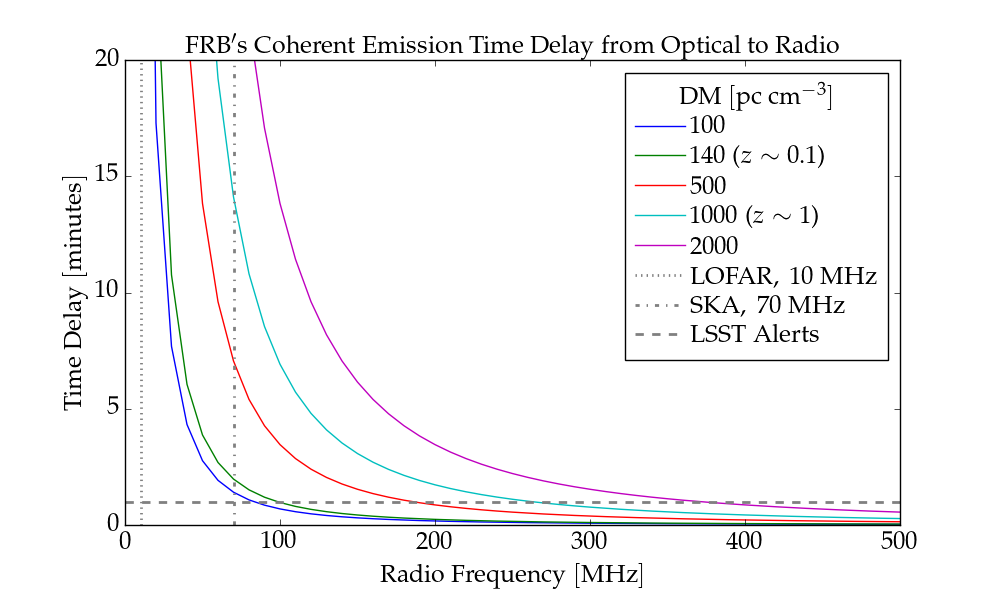
\includegraphics[width=12cm]{figures/frb_optical_delays.png}
\caption{The delay time (for coherent emission) between the arrival of the optical and radio photons due to cosmological dispersion, as a function of the frequency of the radio detector. The {\it lowest} frequency bands of the Square Kilometer Array (SKA\footnote{\url{www.skatelescope.org}}) and the Low-Frequency Array (LOFAR\footnote{\url{lofar.org}}) are marked with vertical dotted and dash-dotted lines, and the 1 minute timescale for LSST alert distribution with a horizontal dashed line. The delay time is $\Delta t = k_{\rm DM}\,DM\,(\nu_{\rm low}^{-2} - \nu_{\rm high}^{-2})$, where $k_{DM}=4.149$ $\rm GHz^2\ pc^{-1}\ cm^3\ ms$, ${\rm DM}$ is the dispersion measure in $\rm pc\ cm^{-3}$, $\nu$ is the low and high frequency bands of the observation, and $\Delta t$ is in $\rm ms$. We have used the range of FRB dispersion measures as observed by \cite{2018Natur.562..386S}. \label{fig:sci_frb}}
\end{center}
\end{figure}


\subsection{Summary of Science-Driven Broker Needs and Recommendations.}\label{ssec:sci_sum}

{\it Summarize the science-driven broker needs here, and perhaps also the 'Challenges Faced'. This section could also, e.g., use or modify Gautham's charted needs, or perhaps create as a new table matrix.}

Say something about how the < 5 min timescale will effect the project. 

Based on these science requirements, we make the following recommendations: 

\nrec
%{System}{Audience}{Phase}
{alerttimescale}
{Understand if there are any scientific uses cases requiring < 5min access to the alerts}
{What, if any, are the driving use cases for access to alerts in < 5 min}

